\chapter{Introduction}

The field of computer science have reached an era where further boost in
single-threaded performance is increasingly complex. Even though Moore's law
\cite{moore1965cramming} is still going strong, Dennard scaling
\cite{dennard1974design} has already dropped far out a few years ago.
\autoref{fig:cpuperformance} sketches up the current state of the art, and it is
easy to see that even though the numbers of transistors per chip is still
increasing, single-threaded performance has flatted out along with frequency and
wattage.

\begin{figure}
    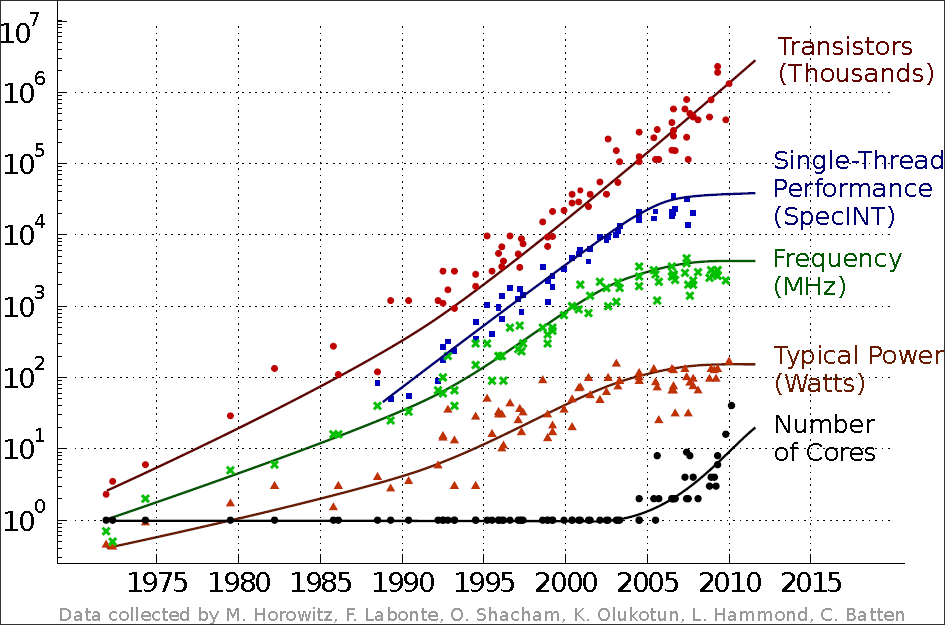
\includegraphics[width=\textwidth]{figs/cpu-performance.png}
    \caption{Historical trends in CPU performance, from \cite{salishan2011}.}
    \label{fig:cpuperformance}
\end{figure}

The reason for this flattening out of performance, frequency and wattage is
mainly because of the Dark Silicon Effect \cite{esmaeilzadeh2011dark}, the
phenomenon of too high power density to be able to cool down a fully powered
chip with ordinary cooling solutions. Where earlier designs exploited a higher
transistor count by adding faster, but more complex components to their designs,
this is no longer possible as it would create too much heat.

\section{Introduction and Motivation}

When faster hardware can no longer be created by just adding more
logic, engineers have to look for more energy efficient solutions
in order to keep power density down. Current research consists of
many branches reaching from homogeneous processors to heterogeneous
systems with loads of interconnect.

\begin{figure}
\begin{subfigure}[b]{0.48\textwidth}
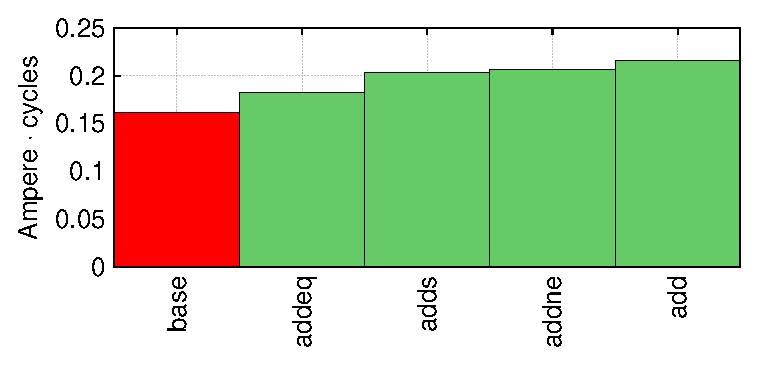
\includegraphics[width=\textwidth]{graph_01_base_cond-0c6.eps}
\caption{Conditional execution (eq is false).}
\end{subfigure}
\begin{subfigure}[b]{0.52\textwidth}
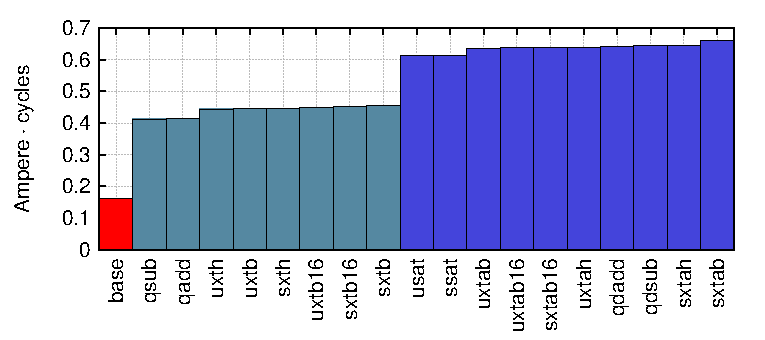
\includegraphics[width=\textwidth]{graph_023_base_quad_saturate_extend-0c6.eps}
\caption{Non-multiply multi-cycle instructions.}
\end{subfigure}
\caption{Figures from \cite{rundehvatum2013exploring} showing the results of measuring the
current drain through the CPU core while running isolated instructions in a loop.}
\end{figure}


\section{Historical Perspective}


Throughout the 80's and 90's, the increasing demand for performance was met by
increasing the clock frequency. Shortening the critical path and exploiting
instruction level parallelism allowed the CPU to run at higher clock speeds to
improve performance \cite{tanenbaum1984structured}. Consequently, processor
manufacturers were able to double single-threaded performance approximately
every 18th month \cite{moore1965cramming}. The tradeoff, however, was an
increased amount of complex logic added complexity to the processor core.
Greater complexity required a greater amount of transistors which must fit on
the same die, made possible by the reduction of transistor size. For a long
time, new process technologies allowed for smaller and less energy consuming
transistors, but as we approached the end of Dennard scaling
\cite{dennard1974design,esmaeilzadeh2011dark}, the amount of logic required to
accomodate speedups could not fit on the die due to thermal constraints. Heat
generation on-chip became overwhelming and one could not simply increase the
frequency or add extra logic to gain additional performance.

\begin{figure}
    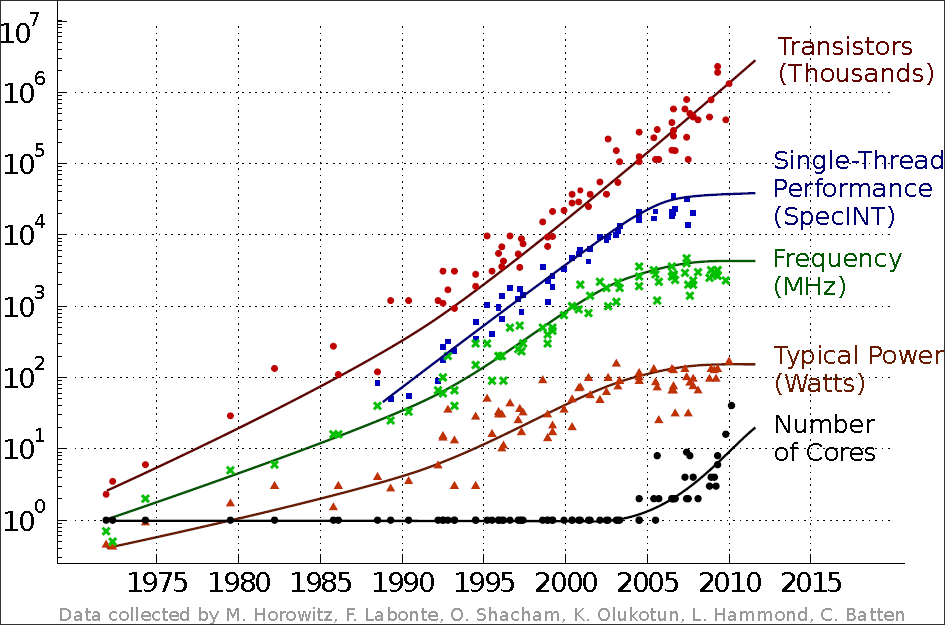
\includegraphics[width=\textwidth]{figs/cpu-performance.png}
    \caption{Historical trends in CPU performance, from \cite{salishan2011}}
    \label{fig:cpuperformance}
\end{figure}

The tremendous growth in performance is depicted in
\autoref{fig:cpuperformance}. We note that although the transistor count is
steadily increasing, single-threaded performance has only seen a minor increase
the last few years.





\section{Demand for Energy Efficiency}

We are now at the beginning of an era where energy efficiency and performance
are tightly coupled. When improving performance, one must take care not to
exceed the physical limitation of power dissipation. Thus, energy efficiency is
key to additional performance gain; performance per Watt must be emphasized.

Heat is not the only motivating factor to keep energy consumption down.
Processors targeting laptops, cellphones and other mobile devices have always
been energy-constrained due to their use of batteries. Lower energy consumption
would allow for longer battery life and/or heavier applications. More recently,
mobile processors have become increasingly popular in alternative domains,
such as supercomputing. Their low cost and high performance per Watt ratio makes
them attractive for massively parallel problems, which is currently done on
large and expensive supercomputers. These machines have huge energy budgets and
are taken out of service after just a couple of years, being replaced by new
machines that offer better performance for less power. Building data centers
from low-cost embedded processors is believed to have a huge potential and
could change the landscape of supercomputing in the future
\cite{rajovic2013supercomputing}.

Not only data centers benefit from the use of mobile processors. The SHMAC
research project at NTNU aims to build a single-ISA heterogeneous computing
platform with processing cores specialized for energy efficiency. Using the most
efficient processor or hardware accelerator -- in terms of both energy and
performance -- is the key to success for such platforms.

There are several reasons to minimize a processors energy consumption. Batteries
would last longer, applications become richer and it will enable processor
performance growth to continue. Energy efficiency has become crucial;
performance alone is no longer the single most important attribute of
processors.


\section{Optimizing for Energy Efficiency}

Given the advanced tools used to support hardware design these days, it is more
easy than ever to model and simulate performance of an unimplemented
architecture. However, modeling power consumption is a much more elaborate
process: Current techniques works on a very low level and uses circuit-level
models to obtain energy metrics. This makes them accurate, but also heavy and
time consuming to simulate. Being able to rapidly prototype and visualize how
changes in the microarchitecture affects energy performance is a key to build
energy efficient hardware as well as an important metric at the design stage. Some
solutions already exists, but most of them inspect energy consumption at very
fine granularity and requires ASIC synthesis of HDL code to work. During the
design process, there is a great need for tools that help developers predict
the changes in power consumption when new features are implemented.

The immediate lack of a system that is easy to use and easy to set up motivates
the creation of a new high-level tool. We introduce PET; a tool that is able to
estimate power usage per time for a given workload on a given architecture. It
will use an energy metric profile estimated from similar processors together
with a simulator trace log to calculate energy usage. Using this approach, PET
will be able to detect if hardware modifications done to the simulation level
model will be beneficial in the realized hardware. PET will also tell if a
processor-implementation is more energy efficient than an other given a specific
workload, thus it can help building workload optimized tiles for the SHMAC
project \cite{shmacwebpage}. Using the features of PET, one can also adjust the
energy metric profile and simulate power usage as if one component was cheaper
or more expensive to use (in terms of energy). This will enable hardware designers to
understand which optimizations are most beneficial and identify possible routes
of exploration in their journey of processor energy optimization.

% SHMAC, power profiles. Velg beste kjerne for gitt workload/application

% TODO: Introduce the notion of 'energy profiles', i.e. energy/time graphs

% motivation: early design stage, check architectural differences using same
% characteristics or set different weights to spesific events in the hunt for
% which components that needs optimization

\section{Assignment Interpretation}

Based on the assignment description text, the following main tasks were
identified.

\begin{description}
    \item[Task 1:] Quantify the exact cost of executing specific instructions on
        a modern out-of-order CPU core
    \item[Task 2:] Create a software suite that sheds light on the energy
        consumption during software execution on various hardware
\end{description}

As can be seen, the problem is twofold. \textit{Task 1} involves performing energy
measurements on hardware components to obtain numbers of a processors energy
characteristics. \textit{Task 2} depends on the results from the former and can
be solved after the completion of \textit{Task 1}.

The first task was solved as a part of the specialization project (TDT4501)
during the fall of 2013, and the final report in its entirety is attached in
\autoref{RH13}. The review of \textit{Task 2} is the main emphasis of this
master's thesis.

\section{Report Organization}

\begin{description}
    \item[Chapter 1: Introduction] provides a historical perspective to the
        trends in processor design and motivates the need for energy efficient
        hardware.
    \item[Chapter 2: Background] contains supportive material on subjects used
        throughout this thesis, as well as explanations that justify decisions
        made later in the report.
    \item[Chapter 3: Building a Power Estimation Tool] is the main piece of our
        problem solution. It contains an in-detail review of what PET does and
        how it is built.
    \item[Chapter 4: PET Performance Tuning] describes considerations needed
        when porting the use of PET to support new hardware configurations.
    \item[Chapter 5: Experiments and Results] presents the tests used to
        evaluate PET, along with accuracy and performance data.
    \item[Chapter 6: Conclusion and Further Work] provides the concluding remarks on the work
        described in this thesis and suggests possible areas of interest for
        further research.
\end{description}


